\chapter{MVVM 模式与 Reactive Programming}

本章将用一定的篇幅详细介绍 MVVM 模式在面向对象的过程式编程语言内的设计实现。使用实例解释 Reactive Programming 以及 FRP 的特性,并导出基于 FRP 进行的 ViewModel 实现。

\section{面向对象的 MVVM 实现}

ViewModel 在 View 与 Model 中间进行数据处理、转换,是 MVVM 模式中的重要角色。

\begin{figure}[!h]
  \begin{center}
    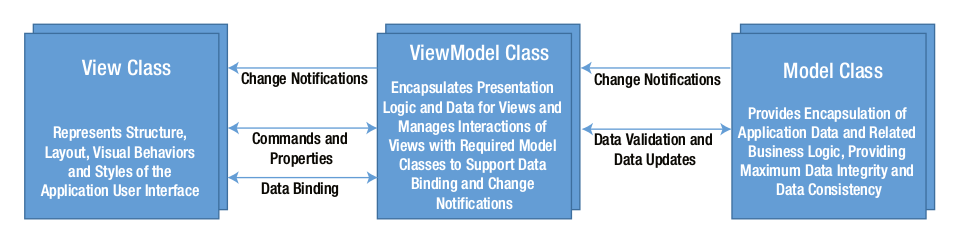
\includegraphics[scale=0.5]{figures/diagram-mvvm-pattern-ref.png}
    \caption{MVVM 设计模式中的关键类~\cite{ghoda2012windows}\label{MVVMCoreClasses}}
  \end{center}
\end{figure}

面向对象的实现中 ViewModel 对象是对观察者模式(Observer Pattern)的一种实现。

\begin{figure}[!h]
  \begin{center}
    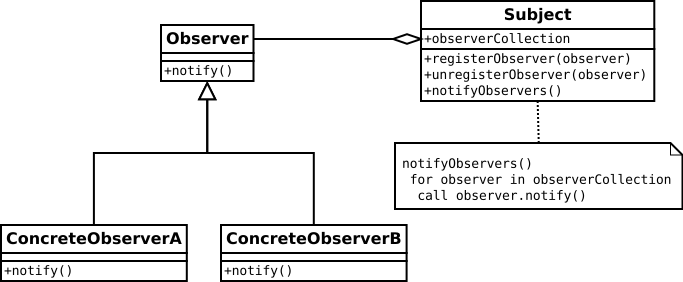
\includegraphics[scale=0.5]{figures/pattern-observer.pdf}
    \caption{观察者模式\label{PatternObserver}}
    Subject 接受注册 Observer 并在 notifyObserver 中向 Observer 推送数据
  \end{center}
\end{figure}

参照类图\footnote{Wikipedia: File:Observer.svg}中的定义对 Model 与 ViewModel 进行定义:

\begin{verbatim}
    @interface IModel implements ISubject;
    @interface IViewModel implements IObserver;
\end{verbatim}

为了让 ViewModel 具有 Model 的特性,将 ViewModel 的接口改写为:

\begin{verbatim}
    @interface IViewModel implements IObserver, IModel;
\end{verbatim}

\begin{figure}[!h]
  \begin{center}
    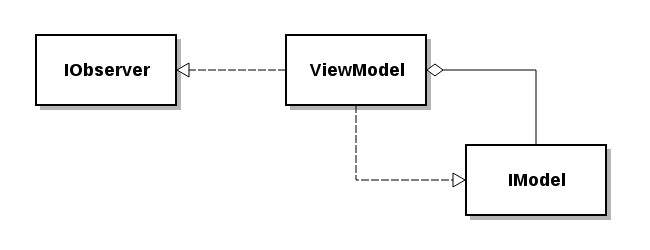
\includegraphics[scale=0.5]{figures/diagram-viewmodel.png}
    \caption{ViewModel 类图\label{ViewModelClass}}
  \end{center}
\end{figure}

ViewModel 通过订阅 Model 获取 Model 的数据变更(图~\ref{MVVMCoreClasses} 中 Model 至 ViewModel 的 $Change Notifications$)。与之类似,View 与 ViewModel 之间的 Binder 定义:

\begin{verbatim}
    @interface IBinder implements ISubject, IObserver;
\end{verbatim}

Binder 实例构造时指定 View 元素作为 Observer 实例,指定 ViewModel 元素作为 Subject 实例就可以建立 ViewModel 至 View 的单向绑定关系。双向绑定关系由两个单项绑定构成,不加赘述。

值得一提的是,由于 ViewModel 同时实现了 Model 接口,具备了 Model 的行为特性,ViewModel 之间也是可以互相观察的:

\begin{figure}[!h]
  \begin{center}
    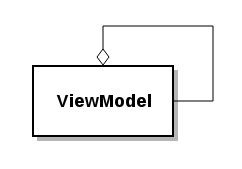
\includegraphics[scale=0.5]{figures/diagram-viewmodel-cascading.png}
    \caption{ViewModel 的可级联特性\label{ViewModelCascading}}
  \end{center}
\end{figure}

这样的设计使得ViewModel模式获得了很强的可扩展性,将用户交互状态分开给不同的 ViewModel 进行管理可以显著减小业务逻辑状态的维护难度,开发者可以利用封装的 ViewModel 类库进行组合来完成用户交互逻辑的实现,具有很高的可复用性。使用 ViewModel 进行开发也同时带来了良好的可测试的代码结构。

通过上面的分析可以看出,观察者模式是 MVVM 模式的重要基础。下一节~\ref{sec:AsyncProgrammingModel} 从编程模型的角度讨论使用观察者模式的合理性并引出FRP作为异步编程模型的解决方案。

\section{用户交互与异步编程模型\label{sec:AsyncProgrammingModel}}

用户与计算机的交互是基于人机交互界面(UI)进行的,早期的终端用户界面 (Console User Interface, CUI) 程序与用户进行同步交互,交互的模型为: 用户输入-程序执行-程序输出-用户输入\ldots,这样的逻辑在面向过程编程的语言实现中是非常自然的程序表达——按先后顺序执行每一条语句。

在图形界面(Graphical User Interface, GUI)得到应用之后,用户可以不间断地与程序进行交互而不需要等待程序的执行,这样的设计极大的提升了用户体验。现代的 GUI 程序广泛使用了事件模型处理用户交互,事件是一组时间顺序的离散数据的集合,对程序来说事件是一类异步产生的数据,因此,基于事件进行编程便成为了进行用户交互实现的基本方法。

明确了这点之后,我们可以将行用户交互实现的本质问题归结为~\textbf{处理异步事件}。

基于事件的开发并不是命令式(Imperative)编程模式所擅长的领域,也导致了大多数 GUI 程序的交互实现都极其不易维护。

以 Drag'n'Drop (拖放操作, DnD) 为例\cite{Zhao2010},在 GUI 上实现 DnD 操作需要程序监听三个不同的 GUI 事件:

\begin{itemize}
  \item 在 MouseDown 事件中标记 isDragging (正在拖动)
  \item 在 MouseMove 事件中判断 isDragging 并且开始绘制拖放光标、使用 API 获取拖放的数据
  \item 在 MouseUp 事件中判断 isDragging 并结束拖放状态(停止绘图)
\end{itemize}

在命令式编程语言中往往使用回调函数(Callback Function)对事件进行处理,这种离散的逻辑碎片导致了在 GUI 实现中出现大量的碎片代码以及全局状态,破坏了“代码逻辑局部性”、“变量局部性”等有利于代码组织和维护的性质。

鉴于这种直接使用回调函数编程的弊端,面向对象的命令式编程语言使用观察者模式(Observer Pattern),利用观察者响应事件数据从而实现对代码的封装管理。

\begin{verbatim}

    @class DnDObserver implements IObserver
      private boolean isDragging;
      private Coord   prevCursorPosition;
      public void notify(propName, oldValue, newValue);

    @interface ObservableView implements ISubject

\end{verbatim}

$ObservableView$ 将事件抽象为一系列数据以及对属性变更事件的触发,$DnDObserver$ 监听 $ObservableView$ 的属性变更,这样的实现维护方便、有较强的可复用性。

异步事件的处理逻辑符合声明式(Declaritive)语言自然的表达方式,使用声明式语言进行用户交互实现的尝试也越来越多。下一节将介绍的的 FRP 方法在异步事件处理方面就有非常出色的性能。

\section{Reactive Programming 与 Monad 函数}

Reactive Programming 的概念继承自 FRP,随着越来越多的语言融入和函数式语言的开发方法,Reactive 模式也被越来越多的应用在 GUI 应用的开发中~\footnote{http://www.reactivemanifesto.org/}。

以 Reactive.js~\footnote{此处使用的是 Reactive.js 的最小 Reactive 核心} 为例~\cite{Carkci2013}

\begin{verbatim}

    // Declaration
    var A = $R(function (b, c) { return b + c });
    var B = $R.state(2); // Initial value for B
    var C = $R.state(1); // Initial value for C
    A.bindTo(B, C); // Declare B and C as argument for A

\end{verbatim}

上面的代码片段演示了 $A = B + C$ 的 Reactive 定义(使用 JavaScript 语言环境),当更改 $B$ 或 $C$ 的值发生改变时 $A$ 的值便会“自动”重新计算。

\begin{verbatim}

    // Reaction
    A();   // -> 3
    B(5);  // Set B to 5
    A();   // -> 6

\end{verbatim}

Reactive 定义中出现的 $\$R$ 函数所产生的对象(即 A、B和C)在纯函数式编程语言中被命名为 Monad~\cite{raey}。

FRP 的将系统抽象为 $行为(Behaviors)$ 和 $事件(Events)$,上例中先使用 Monad 函数包装行为(见 A、B、C 的定义)并在行为之间建立关联(上例中使用 $bindTo$),然后通过传入事件($B(5);$) 更改“行为”的值。

不难发现,Monad 与 Observer 模式有非常相似的行为方式,而且对于具有丰富函数式开发能力的 JavaScript 来说 Monad 能带来更清晰简洁的过程描述。

\section{小结}

本章讨论分析了面向对象 MVVM 模式实现的基础模式——Observer 模式,并举例说明了 Observer 模式在处理异步事件方面较传统的过程式实现方法所具有的优势。

本章还通过实例分析了 Reactive Programming 中 Monad 的应用,详细说明了 Monad 的行为以及与 Observer 的相似性,本项目实现 MVVM 架构的过程中将应用 Monad 结构对 ViewModel 进行开发。

